%Encoding: utf8
%Author: Pavol Loffay, xloffa00@stud.fit.vutbr.cz
%Data: 1.4.2011
%Project: Projekt 3. do predmetu ITY (FIT VUTBR)

%Základní informace o dokumentu
%------------------------------
%rozměry stránky: A4
%rozměry textové oblasti: 17x24cm
%mezera vlevo: 2cm
%mezera nahoře: 3cm
%font: times 11pt

%Překlad
%---------------
%Pro překlad použijte makefile a příkazy latex, dvips a ps2pdf.

%Text k vysázení
%---------------

\documentclass[11pt,a4paper,titlepage]{article}

%preambule
\usepackage[czech]{babel}
\usepackage[top=3.0cm, left=2.0cm, text={17cm, 24cm}]{geometry}
\usepackage[IL2]{fontenc}
\usepackage[utf8]{inputenc}

\usepackage{times}
\usepackage[noline,ruled,longend,czech,algo2e]{algorithm2e}
\usepackage{graphics}

\SetKwFor{For}{for}{do}{end~for}

%dokument
\hyphenation{Příklad}

\begin{document}

\begin{titlepage}
	\begin{center}
		{\Huge \textsc{Vysoké učení technické v~Brně\\}}
		{\huge \textsc{Fakulta informačních technologií\\}}
		\vspace{\stretch{0.382}}
		\bigskip
		{\LARGE Typografie a publikování\,--\,3. projekt\\}
		%\medskip
		{\Huge Tabulky a obrázky\\}
		\bigskip
		\vspace{\stretch{0.618}}	
	\end{center}
	\Large{\today \hfill Pavol Loffay}
	\bigskip
\end{titlepage}

\section{Tabulky}
	Pro sázení tabulek můžeme použít buď prostředí\texttt{ tabbing }nebo prostředí\texttt{ tabular}.

	\subsection{Prostředí\texttt{ tabbing}}
		Při použití \texttt{tabbing} vypadá tabulka následovně:
	\begin{tabbing}
		\textbf{Ovoce} \hspace{16mm}	\= \textbf{Cena} 	\quad 	\=  \textbf{Množství} \\
		Jablka							\> 25,90 					\> 3 kg\\
		Hrušky							\> 27,40					\> 2,5 kg\\
		Vodní melouny					\> 35,--					\> 1 kus \\
	\end{tabbing}

	\noindent Toto prostředí se dá také použít pro sázení algoritmů, ovšem vhodnější je použít 
	prostředí\texttt{ algorithm }nebo\texttt{ algorithm2e }(viz sekce \ref{algoritmy}).

	\subsection{Prostředí\texttt{ tabular}}
		Další možností jak vytvořit tabulku je použít prostředí\texttt{ tabular}. Tabulky pak budou vypadat takto:
		\bigskip

		\begin{table}[h]
			\begin{center}
				\begin{tabular}{|l|r|r|} \hline
							& \multicolumn{2}{|c|}{\textbf{Cena}} \\ \cline{2-3}
					\textbf{Měna} & 	\textbf{nákup} & \textbf{prodej}  \\ \hline 
						EUR & 24,501 & 24,324 \\
						JPY & 105,484 & 105,847 \\
						USD &  16,632 & 16,328 \\ \hline
				\end{tabular}

				\caption{Tabulka kurzů k dnešnímu dni}
				\label{tabulka1}
			\end{center}
		\end{table}

		\begin{table}[h]
			\begin{center}
				\catcode`\-=12
				\begin{tabular}{|c|c|} \hline
					$A$ & $\neg A$ \\ \hline
					\textbf{P} & N \\ \hline
					\textbf{X} & X \\ \hline
					\textbf{N} & P \\ \hline
				\end{tabular}
				\begin{tabular}{|c|c|c|c|c|} \hline
					\multicolumn{2}{|c|}{} & \multicolumn{3}{|c|}{$B$} \\ \cline{3-5}
					\multicolumn{2}{|c|}{$A \wedge B$} & \textbf{P} & \textbf{X} & \textbf{N} \\ \hline
					& \textbf{P} & P & X & N \\ \cline{2-5}
					$A$ & \textbf{X} & X & X & N \\ \cline{2-5}
					& \textbf{N} & N & N & N \\ \hline
				\end{tabular}
				\begin{tabular}{|c|c|c|c|c|} \hline
					\multicolumn{2}{|c|}{} & \multicolumn{3}{|c|}{$B$} \\ \cline{3-5}
					\multicolumn{2}{|c|}{$A \vee B$} & \textbf{P} & \textbf{X} & \textbf{N}\\ \hline
					& \textbf{P} & P & P & P \\ \cline{2-5}
					$A$ & \textbf{X} & P & X & X \\ \cline{2-5}
					& \textbf{N} & P & X & N \\ \hline
				\end{tabular}
				\begin{tabular}{|c|c|c|c|c|} \hline
					\multicolumn{2}{|c|}{} & \multicolumn{3}{|c|}{$B$} \\ \cline{3-5}
					\multicolumn{2}{|c|}{$A \rightarrow B$} & \textbf{P} & \textbf{X} & \textbf{N} \\ \hline
					& \textbf{P} & P & X & N \\ \cline{2-5}
					$A$ & \textbf{X} & P & X & X \\ \cline{2-5}
					& \textbf{N} & P & P & P \\ \hline
				\end{tabular}
				\caption{Kleeneho trojhodnotová logika}
				\label{tabulka2}
			\end{center}
		\end{table}

\section{Algoritmy}
	\label{algoritmy}
	Pokud budeme chtít vysázet algoritmus, můžeme použít prostředí\texttt{ algorithm }nebo\texttt{ algorithm2e}.
	Příklad použití prostředí\texttt{ algorithm2e} viz Algoritmus \ref{algoritmus1}.\\

	Pro nápovědu, jak zacházet s prostředím\texttt{ algorithm }můžeme zkusit tuhle stránku:\\
	http://ftp.cstug.cz/pub/tex/CTAN/macros/latex/contrib/algorithms/algorithms.pdf. \\
	Pro\texttt{ algorithm2e }zase tuhle:\\
	http://www-hep2.fzu.cz/tex/texmf-dist/doc/latex/algorithm2e/algorithm2e.pdf.\\

	\begin{algorithm2e}[H]
		\dontprintsemicolon
		\linesnotnumbered
		\textbf{Input:} \ Množina částic $X$ v čase $t-1$, řízení $u$ v čase $t$ a měření $z$ v čase $t$.\\
		\textbf{Output:} \ Množina částic $X$ v čase $t$. $\overline{X_{t}}=X_{t}=0$\\
		\BlankLine
		\Indp{
			\For{$m=1$ \textup{to} $M$} {
				sample $x_{t}^{[m]} \approx p(x_{t}\ |\ u_{t},x_{t-1}^{[m]})$ \\
				$w_{t}^{[m]} = p(z_{t}\ |\ x_{t}^{[m]})$ \\
				$\overline{X_{t}} = \overline{X_{t}} + \langle x_{t}^{[m]}, w_{t}^{[m]}\rangle$\\ 
			}
			\For{$m=1$ \textup{to} $M$}{
				draw $i$ with probability $\approx w_{t}^{[i]}$ \\
				add $x_{t}^{[i]}$ to $X_{t}$
			}
		\Return $X_{t}$
		}
		\caption{$Particle filter$}
		\label{algoritmus1}
	\end{algorithm2e}

\section{Obrázky}
	Do našich článků můžeme samozřejmě vkládat obrázky. Pokud je obrázkem fotografie,
	můžeme klidně použít bitmapový soubor. Pokud by to ale mělo být nějaké schéma nebo
	něco podobného, je dobrým zvykem takovýto obrázek vytvořit vektorově. \\
	\begin{figure}[h]
		\begin{center}
			\scalebox{0.4}{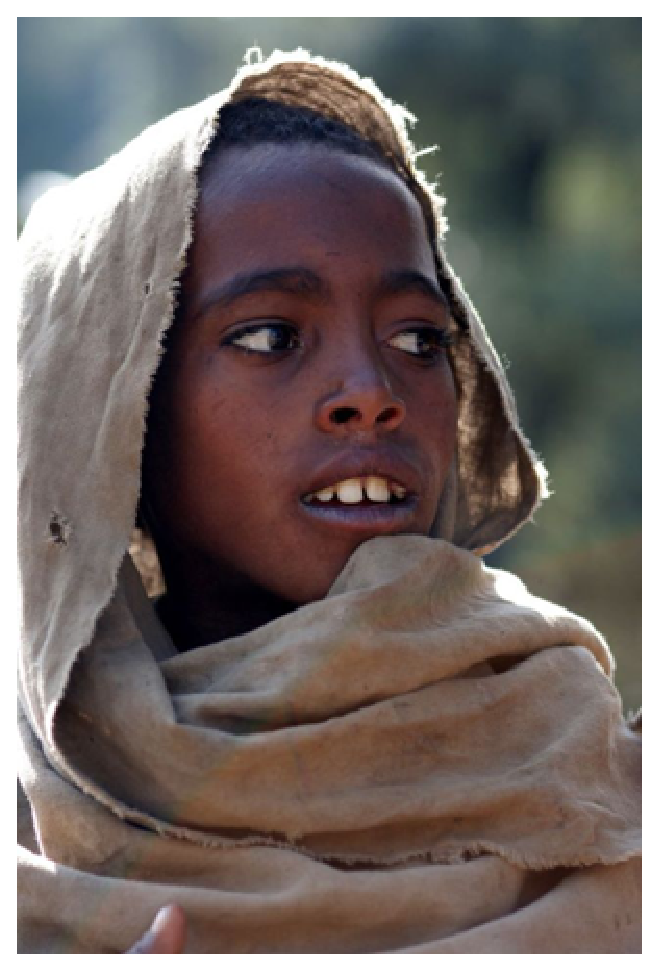
\includegraphics{etiopan.eps}
				\reflectbox{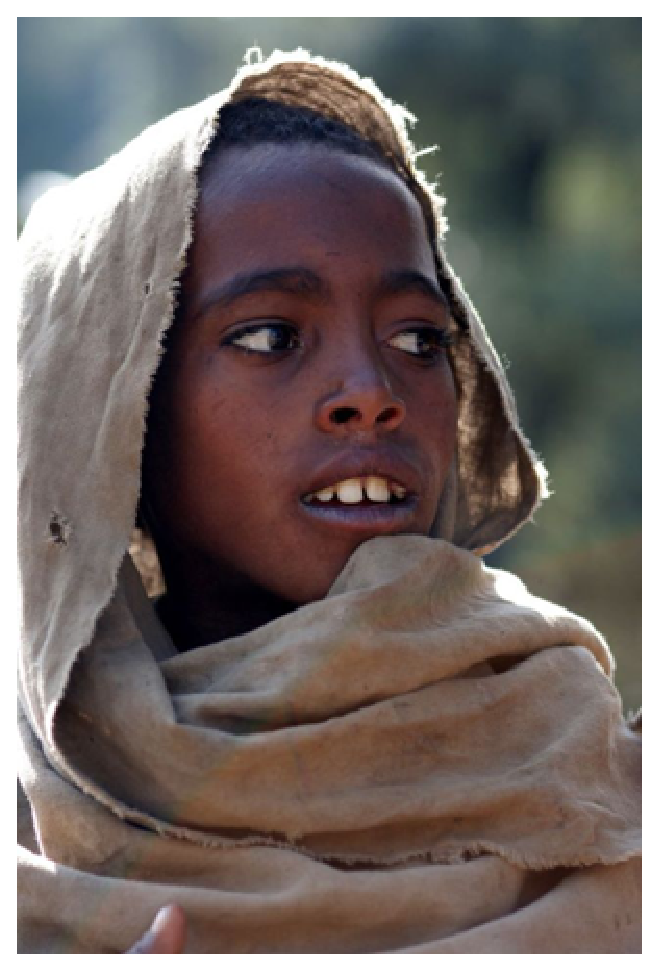
\includegraphics{etiopan.eps}}}
			\caption{Malý etiopánek a jeho bratříček}
			\label{obrazok1}
		\end{center}
	\end{figure}
	\newpage
	Rozdíl mezi vektorovým\,\dots
	\begin{figure}[h]
		\begin{center}
			\scalebox{0.4}{
\includegraphics{oniisan.eps}}
			\caption{Vektorový obrázek}
			\label{obrazok2}
		\end{center}
	\end{figure}

	\noindent\dots\,a bitmapovým obrázkem se projeví například při zvětšení

	\begin{figure}[h]
		\begin{center}
			\scalebox{0.6}{
\includegraphics{oniisan2.eps}}
			\caption{Bitmapový obrázek}
		\label{obrazok3}
		\end{center}
	\end{figure}

	\noindent Tyto odkazy (nejen ty) na obrázky \ref{obrazok1}, \ref{obrazok2} a \ref{obrazok3}, na  
	tabulky \ref{tabulka1} a \ref{tabulka2} a také na algoritmus \ref{algoritmus1} jsou udělány pomocí 
	křížových odkazů. Pak je ovšem potřeba zdrojový soubor přeložit dvakrát.

	\begin{figure}
		\begin{center}
			\setlength{\unitlength}{4pt}
		
			\begin{picture}(115,158.5)(0,0)
%Najvacsi stvorec
				\put(0,0){\linethickness{1pt}\framebox(115,158.5)[cc]{}}
%ciarkovane ciary
				\multiput(15,151.5)(0,-10){16}{\line(0,1){7}}
				\multiput(0,144)(10,0){11}{\line(1,0){7}}
%"medzera" v lavo
				\put(2.5,93){\makebox(10,5)[]{Mezera = 15}}
				\put(7.5,93){\vector(1,0){7.5}}
				\put(7.5,93){\vector(-1,0){7.5}}
%dolny dlhy vektor
				\put(57.5,3){\vector(-1,0){57.5}}
				\put(57.5,3){\vector(1,0){57.5}}
%pravy dlhy vektor
				\put(112,79.25){\vector(0,-1){79.25}}
				\put(112,79.25){\vector(0,1){79.25}}
%LAVA STRANA VEKTORY
%vyska medzery prva 14.5
				\put(88,151.25){\vector(0,1){7.25}}
				\put(88,151.25){\vector(0,-1){7.25}}
				\put(98,154){\makebox(0,0)[c]{Výška}}
				\put(90,151){\makebox(0,0)[l]{mezery = 14,5}}
%vyska medzery druha 10
				\put(88,139){\vector(0,-1){5}}
				\put(88,139){\vector(0,1){5}}
				\put(98,141){\makebox(0,0)[c]{Výška}}
				\put(90,138){\makebox(0,0)[l]{mezery = 10}}
%vyska hlavicky tretia 10
				\put(88,129){\vector(0,-1){5}}
				\put(88,129){\vector(0,1){5}}
				\put(98,131){\makebox(0,0)[c]{Výška}}
				\put(90,128){\makebox(0,0)[l]{hlavičky = 10}}
%vyska medzery 14 stvrta 
				\put(88,117){\vector(0,-1){7}}
				\put(88,117){\vector(0,1){7}}
				\put(98,119){\makebox(0,0)[c]{Výška}}
				\put(90,116){\makebox(0,0)[l]{mezery = 14}}
%vyska tela 75 piata
				\put(88,72.5){\vector(0,-1){37.5}}
				\put(88,72.5){\vector(0,1){37.5}}
				\put(95,67.5){\makebox(0,0)[c]{Výška}}
				\put(90,64.5){\makebox(0,0)[l]{těla = 75}}
%vyska medzery 15 siesta
				\put(88,27.5){\vector(0,-1){7.5}}
				\put(88,27.5){\vector(0,1){7.5}}
				\put(98,29){\makebox(0,0)[c]{Výška}}
				\put(90,26){\makebox(0,0)[l]{mezery = 15}}
%vyska paty 10 siedma
				\put(88,15){\vector(0,-1){5}}
				\put(88,15){\vector(0,1){5}}
				\put(95,16){\makebox(0,0)[c]{Výška}}
				\put(90,13){\makebox(0,0)[l]{paty = 10}}
%VNUTRO OBRAZKY
%hlavicka
				\put(57.5,137){\vector(-1,0){27.5}}
				\put(57.5,137){\vector(1,0){27.5}}
				\put(57.5,139.5){\makebox(0,0)[c]{Šírka boxu = 55}}
				\put(30,124){\linethickness{1pt}\framebox(55,10){\textbf{Hlavička}}}
%telo
				\put(30,35){\linethickness{1pt}\framebox(55,75){\textbf{Textové tělo}}}
%peta
				\put(30,10){\linethickness{1pt}\framebox(55,10){\textbf{Pata}}}
%vyska stranky 185,5, sikmy vektor
				\put(102,56.5){\vector(1,1){10}}
				\put(102,53.5){\makebox(0,0)[c]{Výška}}
				\put(93,50){\makebox(0,0)[l]{stránky = 158,5}}
%sirka stranky 115  ulne dole
				\put(58,6){\makebox(0,0)[c]{Šířka stránky = 115}}
%sirka boxu 15 
				\put(89.5,93){\vector(1,0){4.5}}
				\put(89.5,93){\vector(-1,0){4.5}}
				\put(101.5,93){\vector(1,0){7.5}}
				\put(101.5,93){\vector(-1,0){7.5}}
				\put(101,98){\makebox(0,0)[c]{Šířka}}
				\put(96,95){\makebox(0,0)[l]{boxu = 15}}
%medzera 9 a sikmy vektor
				\put(97.5,106.5){\makebox(0,0)[c]{Mezera = 9}}
				\put(96,105){\vector(-1,-2){6}} 
%okrajova poznamka
				\put(94,80){\linethickness{1pt}\framebox(15,10){\textbf{\shortstack{Okrajová\\poznámka}}}}
			\end{picture}
		\caption{Vektorový obrázek v prostředí \texttt{picture}}
		\end{center}
	\end{figure}
\end{document}